% !TeX program = xelatex
% Сборка: xelatex report.tex
% Персональные данные для титульного листа изменяются в этом блоке.
\documentclass[14pt,a4paper]{extarticle}

\usepackage{graphicx}
\usepackage{fvextra}
\usepackage{amsmath}
\usepackage{fontspec}
\IfFontExistsTF{Times New Roman}
    {
        \setmainfont{Times New Roman}
        \setsansfont{Times New Roman}
        \setmonofont{Times New Roman}
        \newfontfamily\cyrillicfont{Times New Roman}
        \newfontfamily\cyrillicfontsf{Times New Roman}
        \newfontfamily\cyrillicfonttt{Times New Roman}
    }
    {
        \setmainfont{Liberation Serif}
        \setsansfont{Liberation Serif}
        \setmonofont{Liberation Serif}
        \newfontfamily\cyrillicfont{Liberation Serif}
        \newfontfamily\cyrillicfontsf{Liberation Serif}
        \newfontfamily\cyrillicfonttt{Liberation Serif}
        \PackageWarningNoLine{report}{Times New Roman is not installed;
        using Liberation Serif temporarily}
    }
\usepackage{unicode-math}
\setmathfont{texgyretermes-math.otf}
\usepackage{polyglossia}
\setdefaultlanguage{russian}
\usepackage[left=30mm,right=15mm,top=20mm,bottom=20mm]{geometry}
\usepackage{setspace}
\usepackage{indentfirst}
\usepackage{enumitem}
\usepackage{titlesec}
\usepackage{caption}
\usepackage{float}
\usepackage[section]{placeins}
\usepackage{tabularx}
\usepackage{tikz}
\usetikzlibrary{arrows.meta,positioning}
\usepackage{pgfplots}
\pgfplotsset{compat=1.18}
\usepackage[hidelinks]{hyperref}


\newcommand{\Ministry}{МИНОБРНАУКИ РОССИИ}
\newcommand{\University}{Санкт-Петербургский государственный\\
электротехнический университет\\
«ЛЭТИ» им. В.И. Ульянова (Ленина)}
\newcommand{\Department}{МОЭВМ}
\newcommand{\StudentName}{Пархоменко М.~С.}
\newcommand{\StudentGroup}{2304}
\newcommand{\TeacherName}{Татаринов Ю.~С.}
\newcommand{\City}{Санкт-Петербург}

\setstretch{1.5}
\setlength{\parindent}{1.25cm}
\setlength{\parskip}{0pt}
\setlength{\emergencystretch}{3em}
\titleformat{\section}{\normalfont\bfseries\centering}{\thesection}{0.5em}{}
\titlespacing*{\section}{0pt}{1.5em}{1em}
\titleformat{\subsection}{\normalfont\bfseries}{\thesubsection.}{0.5em}{}
\setlist{nosep,leftmargin=1.25cm}
\captionsetup{
    font=normalsize,
    labelsep=endash,
    skip=6pt
}
\captionsetup[figure]{
    name=Рисунок,
    justification=centering,
    singlelinecheck=false
}
\captionsetup[table]{
    name=Таблица,
    position=top,
    justification=raggedright,
    singlelinecheck=false
}
\newcommand{\sectionbreak}{\clearpage}

\begin{document}

\begin{titlepage}
    \thispagestyle{empty}
    \begin{center}
        \Ministry

        \University

        Кафедра \Department
    \end{center}

    \vspace{2cm}

    \begin{center}
        \textbf{ОТЧЕТ}

        по практической работе №~3

        по дисциплине «Системы параллельной обработки данных»

        \vspace{0.5cm}
        Тема: «Поэлементное суммирование массивов средствами MPI»
    \end{center}

    \vspace{2cm}

    \begin{flushright}
        \begin{minipage}{0.8\textwidth}
            \begin{tabularx}{\linewidth}{@{}p{4.8cm}
                >{\centering\arraybackslash}p{2.8cm} X@{}}
                Студент гр. \StudentGroup
                & \rule{2.5cm}{0.4pt} & \StudentName\\
                & подпись & \\[0.8cm]
                Преподаватель
                & \rule{2.5cm}{0.4pt} & \TeacherName\\
                & подпись &
            \end{tabularx}
        \end{minipage}
    \end{flushright}

    \vfill

    \begin{center}
        \City\\
        2026
    \end{center}
\end{titlepage}

\setcounter{page}{2}

\section{Цель работы}

Изучить коллективную операцию редукции MPI, реализовать поэлементное
суммирование массивов целых чисел и исследовать время выполнения
при изменении числа процессов в соответствии с постановкой задачи.

\section{Формулировка задания}

\textbf{Вариант 7.} В каждом процессе дан набор из $K+5$ целых чисел,
где $K$ — количество процессов. Используя функцию \texttt{MPI\_Reduce}
для операции \texttt{MPI\_SUM}, просуммировать элементы данных наборов
с одним и тем же порядковым номером и вывести полученные суммы в главном
процессе.

\section{Описание алгоритма}

В работе участвуют $K$ процессов с рангами $r=0,\ldots,K-1$.
После \texttt{MPI\_Init} каждый процесс узнаёт свой ранг и число процессов,
создаёт массив длины $n=K+5$ и заполняет его по правилу
\begin{equation}
 a_{r,i}=ir,\qquad 0\leq i<n,
\end{equation}
где $a_{r,i}$ — элемент с индексом $i$ в процессе с рангом $r$.

После вывода исходных массивов выполняется \texttt{MPI\_Barrier}.
Затем все процессы вызывают \texttt{MPI\_Reduce} с одинаковыми
параметрами: число элементов $n$, тип \texttt{MPI\_INT}, операция
\texttt{MPI\_SUM}, корневой процесс 0 и коммуникатор
\texttt{MPI\_COMM\_WORLD}. При передаче массива редукция выполняется
поэлементно, а приёмный буфер значим у корневого процесса~[1].

Процесс 0 выводит массив сумм. Каждый процесс вызывает
\texttt{MPI\_Finalize}. Полный исходный код приведён в приложении А,
а отдельная измерительная версия — в приложении Б.

Для проверки результата используется формула
\begin{equation}
\label{eq:expected}
 b_i=\sum_{r=0}^{K-1}a_{r,i}
     =i\frac{K(K-1)}{2},\qquad 0\leq i<K+5,
\end{equation}
где $b_i$ — элемент результирующего массива с индексом $i$.
При $K=1$ исходный массив нулевой, поэтому результат также нулевой.
Подготовка данных занимает $O(n)$ операций на процесс; каждый процесс
хранит два массива длины $n$. Внутренний способ выполнения редукции
выбирается библиотекой MPI и в исходном коде программы не задаётся~[1].

\section{Формальное описание посредством сети Петри}

Алгоритм представлен цветной сетью Петри на
рисунке~\ref{fig:petri}. Фишка содержит ранг процесса и, при необходимости,
его массив. Начальная маркировка места $I$ содержит $K$ фишек с различными
рангами; она соответствует состоянию после инициализации MPI.
Для описания параллельных процессов
использован аппарат сетей Петри~[2].

\begin{figure}[H]
\centering
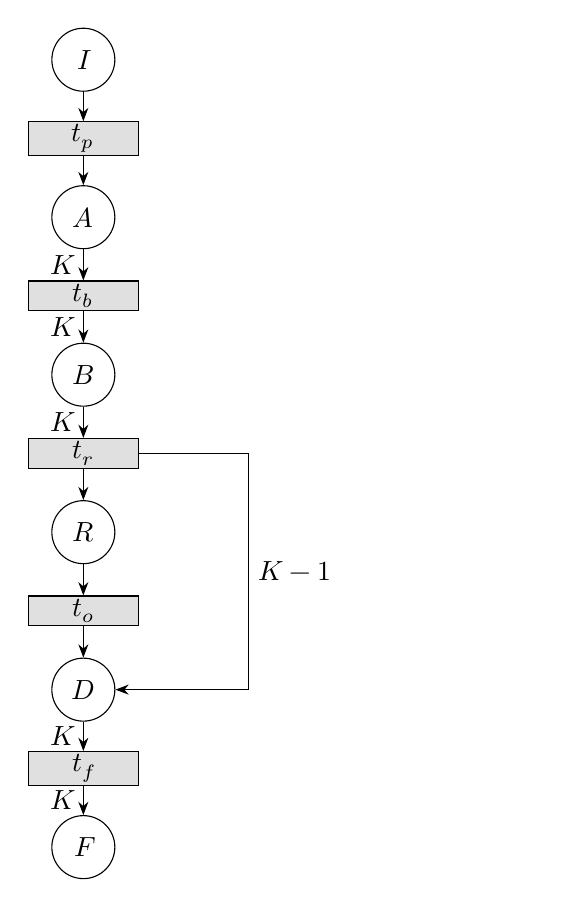
\begin{tikzpicture}[
    >=Stealth,
    place/.style={circle,draw,minimum size=8mm,inner sep=1pt},
    trans/.style={rectangle,draw,fill=black!12,minimum width=14mm,
                  minimum height=3mm,inner sep=1pt},
    every node/.style={font=\normalsize}
]
\node[place] (i) at (0,0) {$I$};
\node[trans] (p) at (0,-1) {$t_p$};
\node[place] (a) at (0,-2) {$A$};
\node[trans] (b) at (0,-3) {$t_b$};
\node[place] (s) at (0,-4) {$B$};
\node[trans] (r) at (0,-5) {$t_r$};
\node[place] (v) at (0,-6) {$R$};
\node[trans] (o) at (0,-7) {$t_o$};
\node[place] (d) at (0,-8) {$D$};
\node[trans] (f) at (0,-9) {$t_f$};
\node[place] (z) at (0,-10) {$F$};
\draw[->] (i) -- (p);
\draw[->] (p) -- (a);
\draw[->] (a) -- node[left] {$K$} (b);
\draw[->] (b) -- node[left] {$K$} (s);
\draw[->] (s) -- node[left] {$K$} (r);
\draw[->] (r) -- (v);
\draw[->] (v) -- (o);
\draw[->] (o) -- (d);
\draw[->] (d) -- node[left] {$K$} (f);
\draw[->] (f) -- node[left] {$K$} (z);
\draw[->] (r.east) -- (2.1,-5) -- node[right] {$K-1$} (2.1,-8) -- (d.east);
\node[anchor=west] at (3,0) {Процессы после инициализации};
\node[anchor=west] at (3,-2) {Локальные массивы готовы};
\node[anchor=west] at (3,-4) {Барьер пройден};
\node[anchor=west] at (3,-6) {Корень получил массив сумм};
\node[anchor=west] at (3,-8) {Готовность к завершению};
\node[anchor=west] at (3,-10) {Программа завершена};
\end{tikzpicture}
\caption{Цветная сеть Петри основной программы}
\label{fig:petri}
\end{figure}

Переход $t_p$ срабатывает отдельно для каждого ранга, остальные
переходы отражают общие этапы или действие корневого процесса.
Функционал переходов приведён в таблице~\ref{tab:transitions}.
Число у дуги означает количество фишек; немаркированная дуга переносит
одну фишку. Ветвь с весом $K-1$ при $K=1$ не создаёт фишек.

\begin{table}[H]
\caption{Функционал переходов сети Петри}
\label{tab:transitions}
\begin{tabularx}{\linewidth}{c|X}
Переход & Действие \\
\hline
$t_p$ & Извлекает фишку ранга $r$ из $I$, формирует и выводит массив
$a_r$, помещает фишку $(r,a_r)$ в $A$. \\
$t_b$ & При наличии всех $K$ фишек из $A$ переносит их в $B$;
моделирует барьер перед коллективной операцией. \\
$t_r$ & Обрабатывает $K$ массивов из $B$, вычисляет $b_i=\sum_r a_{r,i}$;
создаёт фишку $(0,b)$ в $R$ и $K-1$ фишек ненулевых рангов в $D$. \\
$t_o$ & Выводит массив из фишки $(0,b)$ места $R$ и переносит
фишку ранга 0 в $D$. \\
$t_f$ & При наличии $K$ фишек в $D$ переводит модель в конечное
состояние $F$; обозначает завершение программы всеми процессами.
\end{tabularx}
\end{table}

Редукция показана одним укрупнённым переходом, без моделирования
внутренних сообщений библиотеки. Модель отражает результат
операции и не задаёт одновременный выход всех процессов
из \texttt{MPI\_Reduce}. Место $D$ и переход $t_f$ фиксируют завершение
всей программы; дополнительного вызова барьера после редукции в коде нет.

Каждый ранг проходит подготовку один раз и участвует в коллективной
операции. Из $R$ выходит только фишка ранга 0, поэтому вывод массива сумм
выполняется один раз. После обработки корня в $D$ находятся все $K$
рангов, что позволяет достичь конечного состояния.

\section{Примеры работы и проверка корректности}

На рисунке~\ref{fig:run-four} показан запуск на четырёх процессах.
В каждом процессе сформирован массив из девяти чисел.
Сумма рангов равна $0+1+2+3=6$, поэтому по формуле~\eqref{eq:expected}
ожидается массив
\[
(0,6,12,18,24,30,36,42,48).
\]
На скриншоте получен именно этот результат.

\begin{figure}[H]
\centering
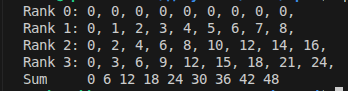
\includegraphics[width=0.92\linewidth]{screenshots/4proc_result.png}
\caption{Исходные массивы и результат на четырёх процессах}
\label{fig:run-four}
\end{figure}

Результаты функциональных проверок представлены в
таблице~\ref{tab:functional}. В этих запусках результаты соответствовали
формуле~\eqref{eq:expected}, программы завершились с кодом 0.

\begin{table}[H]
\caption{Функциональные проверки программы}
\label{tab:functional}
\centering
\begin{tabularx}{\linewidth}{cc|X}
$K$ & $n$ & Полученный массив сумм \\
\hline
1 & 6 & $(0,0,0,0,0,0)$ \\
2 & 7 & $(0,1,2,3,4,5,6)$ \\
4 & 9 & $(0,6,12,18,24,30,36,42,48)$
\end{tabularx}
\end{table}

Порядок строк разных рангов может изменяться. Барьер перед редукцией
ожидает участия всех процессов, но не упорядочивает доставку их вывода
в терминал. Эта особенность не влияет на вычисленные суммы.

\section{Экспериментальное исследование}

\subsection{Методика и условия}

Измерительная версия сохраняет длину массива $n=K+5$.
Подготовка массивов, барьер, инициализация и завершение MPI, а также
печать не включаются в измеряемый интервал. Каждый процесс измеряет
локальное время серии из $L=1000$ вызовов \texttt{MPI\_Reduce}
с операцией \texttt{MPI\_SUM}. Таймер \texttt{MPI\_Wtime} вызывается
непосредственно перед циклом и сразу после него.

Отдельный коллективный вызов с \texttt{MPI\_MAX} собирает максимум
локальных длительностей после остановки таймера. Время одного вызова
в запуске $j$ вычисляется по формуле
\begin{equation}
 T_j(K)=\frac{\max_{0\leq r<K}(t^{\mathrm{end}}_{r,j}
              -t^{\mathrm{start}}_{r,j})}{L}.
\end{equation}
Таким образом, часы разных процессов друг с другом не вычитаются.

Для каждого $K=1,2,4,8,16$ выполнено семь отдельных запусков MPI;
итоговым временем считается медиана семи значений $T_j(K)$.
Прогрев не выполнялся: начальные затраты первых вызовов входят
в длительность серии. В каждой серии повторно обрабатываются одни и те же
буферы; результат перезаписывается и не накапливается между итерациями.

Скрипт \texttt{pr3/scripts/run\_benchmark.py} сохраняет все 35 значений
в CSV, составляет сводную таблицу и записывает параметры окружения.
Пример прогона приведён на рисунке~\ref{fig:benchmark-run}.

\begin{figure}[H]
\centering
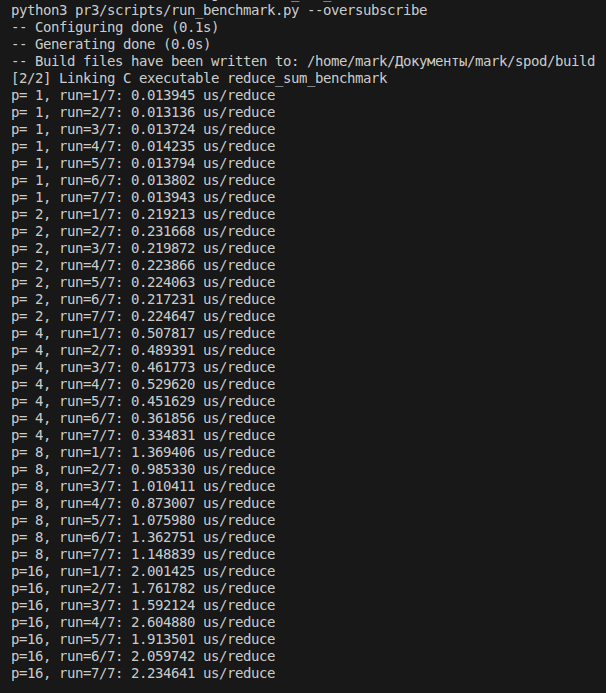
\includegraphics[width=0.80\linewidth,height=0.74\textheight,keepaspectratio]{screenshots/run_benchmark.png}
\caption{Семь запусков бенчмарка для каждого количества процессов}
\label{fig:benchmark-run}
\end{figure}

Согласно сохранённым метаданным использованы Intel Core i3-12100,
восемь логических CPU, Linux 7.0.0-42-generic, Open MPI 4.1.6 и
GCC 13.3.0. Конфигурация CMake — Release, параметры оптимизации
\texttt{-O3 -DNDEBUG}. Запуск выполнялся с параметрами
\texttt{--use-hwthread-cpus --oversubscribe}. При $K=16$ число процессов
превышало число логических CPU, то есть использовалась переподписка.

\subsection{Результаты измерений}

В таблице~\ref{tab:reduce-benchmark} приведены времена одного вызова
в микросекундах. Минимум и максимум характеризуют разброс между семью
запусками, а не времена отдельных итераций внутри серии.
\begin{table}[H]
\caption{Время одной редукции: семь запусков без прогрева, мкс}
\label{tab:reduce-benchmark}
\centering
\begin{tabular}{cc|rrr}
$K$ & $n=K+5$ & Минимум & Медиана & Максимум \\
\hline
1 & 6 & 0,013 & 0,014 & 0,014 \\
2 & 7 & 0,217 & 0,224 & 0,232 \\
4 & 9 & 0,335 & 0,462 & 0,530 \\
8 & 13 & 0,873 & 1,076 & 1,369 \\
16 & 21 & 1,592 & 2,001 & 2,605 \\
\end{tabular}
\end{table}


Зависимость времени от числа процессов показана на
рисунке~\ref{fig:time-processes}. Вертикальные отрезки обозначают минимум
и максимум, точки — медиану. Логарифмическая шкала времени позволяет
показать режим без обмена при $K=1$ и режимы с несколькими процессами.

\begin{figure}[H]
\centering
\begin{tikzpicture}
\begin{axis}[
 width=0.94\linewidth,height=8cm,
 xlabel={Число процессов $K$},ylabel={Время одной редукции, мкс},
 xtick={1,2,4,8,16},ymode=log,grid=major,
 tick label style={font=\small}
]
\addplot+[blue,mark=*,error bars/.cd,y dir=both,y explicit]
 table[col sep=comma,x=processes,y=median_us,
 y error plus expr={\thisrow{max_us}-\thisrow{median_us}},
 y error minus expr={\thisrow{median_us}-\thisrow{min_us}}]
 {../results/reduce_sum_benchmark_summary.csv};
\end{axis}
\end{tikzpicture}
\caption{Время редукции при изменении $K$ и длине массива $n=K+5$}
\label{fig:time-processes}
\end{figure}

На рисунке~\ref{fig:time-size} те же измерения представлены по длине
локального массива. Это не независимая серия по размеру задачи:
каждой длине соответствует своё число процессов.

\begin{figure}[H]
\centering
\begin{tikzpicture}
\begin{axis}[
 width=0.94\linewidth,height=8cm,
 xlabel={Длина локального массива $n$},ylabel={Время одной редукции, мкс},
 xtick={6,7,9,13,21},ymode=log,grid=major,
 tick label style={font=\small}
]
\addplot+[blue,mark=*] table[col sep=comma,x=array_length,y=median_us]
 {../results/reduce_sum_benchmark_summary.csv};
\end{axis}
\end{tikzpicture}
\caption{Время для массивов длины $n=K+5$ при соответствующих $K$}
\label{fig:time-size}
\end{figure}

\subsection{Анализ времени и границы исследования}

В рассмотренных точках медианное время монотонно увеличивалось:
от 0,013802~мкс при $K=1$ до 2,001425~мкс при $K=16$.
При $K=1$ межпроцессной передачи нет; этот режим значительно дешевле
вариантов с несколькими процессами. При переходе от $K=2$ к $K=4$
медиана выросла примерно в 2,06 раза, от $K=4$ к $K=8$ — в 2,33 раза,
от $K=8$ к $K=16$ — в 1,86 раза.

При $K=4$ времена отдельных запусков лежали в диапазоне
0,334831–0,529620~мкс, при $K=8$ — 0,873007–1,369406~мкс.
Разброс показывает, что результат зависит от условий конкретного запуска.
На него могут влиять планирование процессов, начальные затраты и состояние
кешей. Увеличение числа участников добавляет расходы коллективного обмена;
при этом длина локального массива также возрастает с 6 до 21 элемента.
Отдельный вклад каждого фактора по этим данным определить нельзя.

Точка $K=16$ дополнительно включает переподписку. Её нельзя трактовать
как выполнение на шестнадцати независимых аппаратных потоках.
По изменению наклона графика нельзя определить, менялся ли
внутренний алгоритм MPI. Для этого нужны отдельные опыты.

Общие требования предусматривают независимое исследование по числу
процессов и размеру задачи. В текущей программе $n=K+5$, поэтому
получена только одна связанная серия. Для полного исследования нужны
отдельно задаваемые значения $n$, например 16, 1024 и 65536,
с одинаковым набором $K$ для каждого $n$. Эти эксперименты пока не проведены.

\subsection{Ускорение и эффективность}

Для сопоставимых объёмов работы ускорение и эффективность определяются
как
\begin{equation}
 S(K,n)=\frac{T_{\mathrm{seq}}(K,n)}{T_{\mathrm{MPI}}(K,n)},
 \qquad E(K,n)=\frac{S(K,n)}{K},
\end{equation}
где $T_{\mathrm{seq}}(K,n)$ — время последовательного суммирования тех же
$K$ массивов длины $n$, а $T_{\mathrm{MPI}}(K,n)$ — время MPI-варианта
без формирования исходных данных и вывода.

Редукция на одном процессе обрабатывает только один массив и не является
такой последовательной базой. Поэтому отношение измеренного времени
при $K=1$ к времени при $K>1$ не характеризует ускорение одной задачи.
Последовательная база не измерялась: численные значения и графики
$S$ и $E$ по имеющимся данным не строятся. Зону эффективного
распараллеливания на основании этой серии установить нельзя.

\section{Выводы}

Реализовано поэлементное суммирование массивов длины $K+5$
с помощью \texttt{MPI\_Reduce} и \texttt{MPI\_SUM}. Все процессы
участвуют в коллективном вызове, а массив сумм получает и выводит
процесс 0. Проверки при $K=1,2,4$ дали результаты, соответствующие
аналитической формуле. Алгоритм представлен цветной сетью Петри
с описанием функционала переходов.

Время исследовано для $K=1,2,4,8,16$: выполнено по семь запусков,
в каждом измерена серия из 1000 редукций без прогрева. Измеряемый участок
не включает подготовку массивов, вывод и сбор локальных длительностей.
Медиана времени одного вызова возросла с 0,013802 до 2,001425~мкс.
Увеличение числа процессов в этой серии не сопровождалось уменьшением
времени; при 16 процессах использовалась переподписка.

Полученные данные характеризуют текущую постановку со связанными
$K$ и $n$, но не дают независимых зависимостей по двум параметрам.
Для завершения исследования эффективности требуются серии
с независимо заданной длиной массива и измерения сопоставимой
последовательной базы. До их выполнения вывод о наличии или отсутствии
области ускорения не обоснован.

\section{Список использованных источников}

\begin{enumerate}[label={[\arabic*]},leftmargin=1.25cm]
\item MPI Forum. MPI 4.1. Раздел 7.9.1. Reduce. 2023.
\url{https://www.mpi-forum.org/docs/mpi-4.1/mpi41-report/node130.htm}.
\par Дата обращения: 10.11.2026.
\item Мараховский В.~Б., Розенблюм Л.~Я., Яковлев А.~В.
Моделирование параллельных процессов. Сети Петри.
СПб.: Профессиональная литература, 2014.
\end{enumerate}

\clearpage
\phantomsection
\section*{ПРИЛОЖЕНИЕ А\\Листинг основной программы}
\VerbatimInput[fontsize=\normalsize,breaklines=true,breakanywhere=true]{../src/reduce_sum.c}

\clearpage
\phantomsection
\section*{ПРИЛОЖЕНИЕ Б\\Листинг измерительной программы}
\VerbatimInput[fontsize=\normalsize,breaklines=true,breakanywhere=true]{../src/reduce_sum_benchmark.c}

\end{document}
